\subsubsection{Harmonic Analysis applied to Communications
               Engineering}\label{ict:pfander}
               \index{Pfander, G\"otz}

\paragraph{Research Team}
G\"{o}tz Pfander (Professor), Niklas Grip (Postdoctoral Fellow)\\

%%% give a very short (150 words description of your research area)

In Multi-Carrier Modulation (MCM) communication schemes, the
channel input signal is synthesized as a linear combination
(superposition) of certain basis functions whose coeffcients
(weights) are bearing digital information. The performance of an
MCM system depends largely on the choice of the basis functions
which should allow the receiver to perform a fast and reliable
recovery of the transmitted information from the channel output.

For years, Orthogonal Frequency Division Multiplexing (OFDM) has
dominated MCM transmission systems, originally in time invariant
environments as in DSL applications but more recently also in slowly
time varying channels. The reason for this lies in the fact that, in
the stationary set-up, the OFDM carrier signals are approximate
eigenfunctions of the channel operator.

Mathematically, or more precisely, within harmonic analysis, OFDM
has been extensively studied under the disguise of Gabor analysis,
where stability issues, synthesis and analysis algorithms, and
carrier functions design are discussed at length (see also
Section~\ref{mps:pfander}).


\paragraph{Highlights}

In recent years, we have applied Gabor analysis to provide
mathematical contributions to MCM communications. For example, we
have shown that Gabor systems (OFDM, DMT) clearly outperform wavelet
systems (DWMT) in time invariant channels and we have analyzed
estimates of the crest factor of trigonometric polynomials which
underly OFDM.

In mobile and therefore wireless and time variant communication
environments, the transmitted signal reaches the receiver along a
continuum of different signal paths, each featuring a path dependent
time delay and a frequency shift caused by the doppler effect.
Nevertheless, physical constraints imply that this time--frequency
dispersion of the transmission signal is of limited extent. Hence,
wireless channels can be modelled by operators, which are weighted
superpositions of time and frequency shifts occupying a limited
region, the so--called spreading support in the time--frequency
plane. The weight functions are the so--called spreading functions
which play a fundamental role in our research
(Section~\ref{mps:pfander}).

\null {\emph{Transmission Basis Design:}} Since Fall 2004, we are
working on a DFG funded project, whose aim is the mathematical
analysis and optimisation of coded orthogonal frequency division
multiplexing (COFDM) in view of transmission stability in wireless
and other time variant environments. One of the cornerstones of
this project is the analysis of the perturbation stability of
different bases when used in wireless channels.

 \begin{figure}[ht]
   \begin{center}
    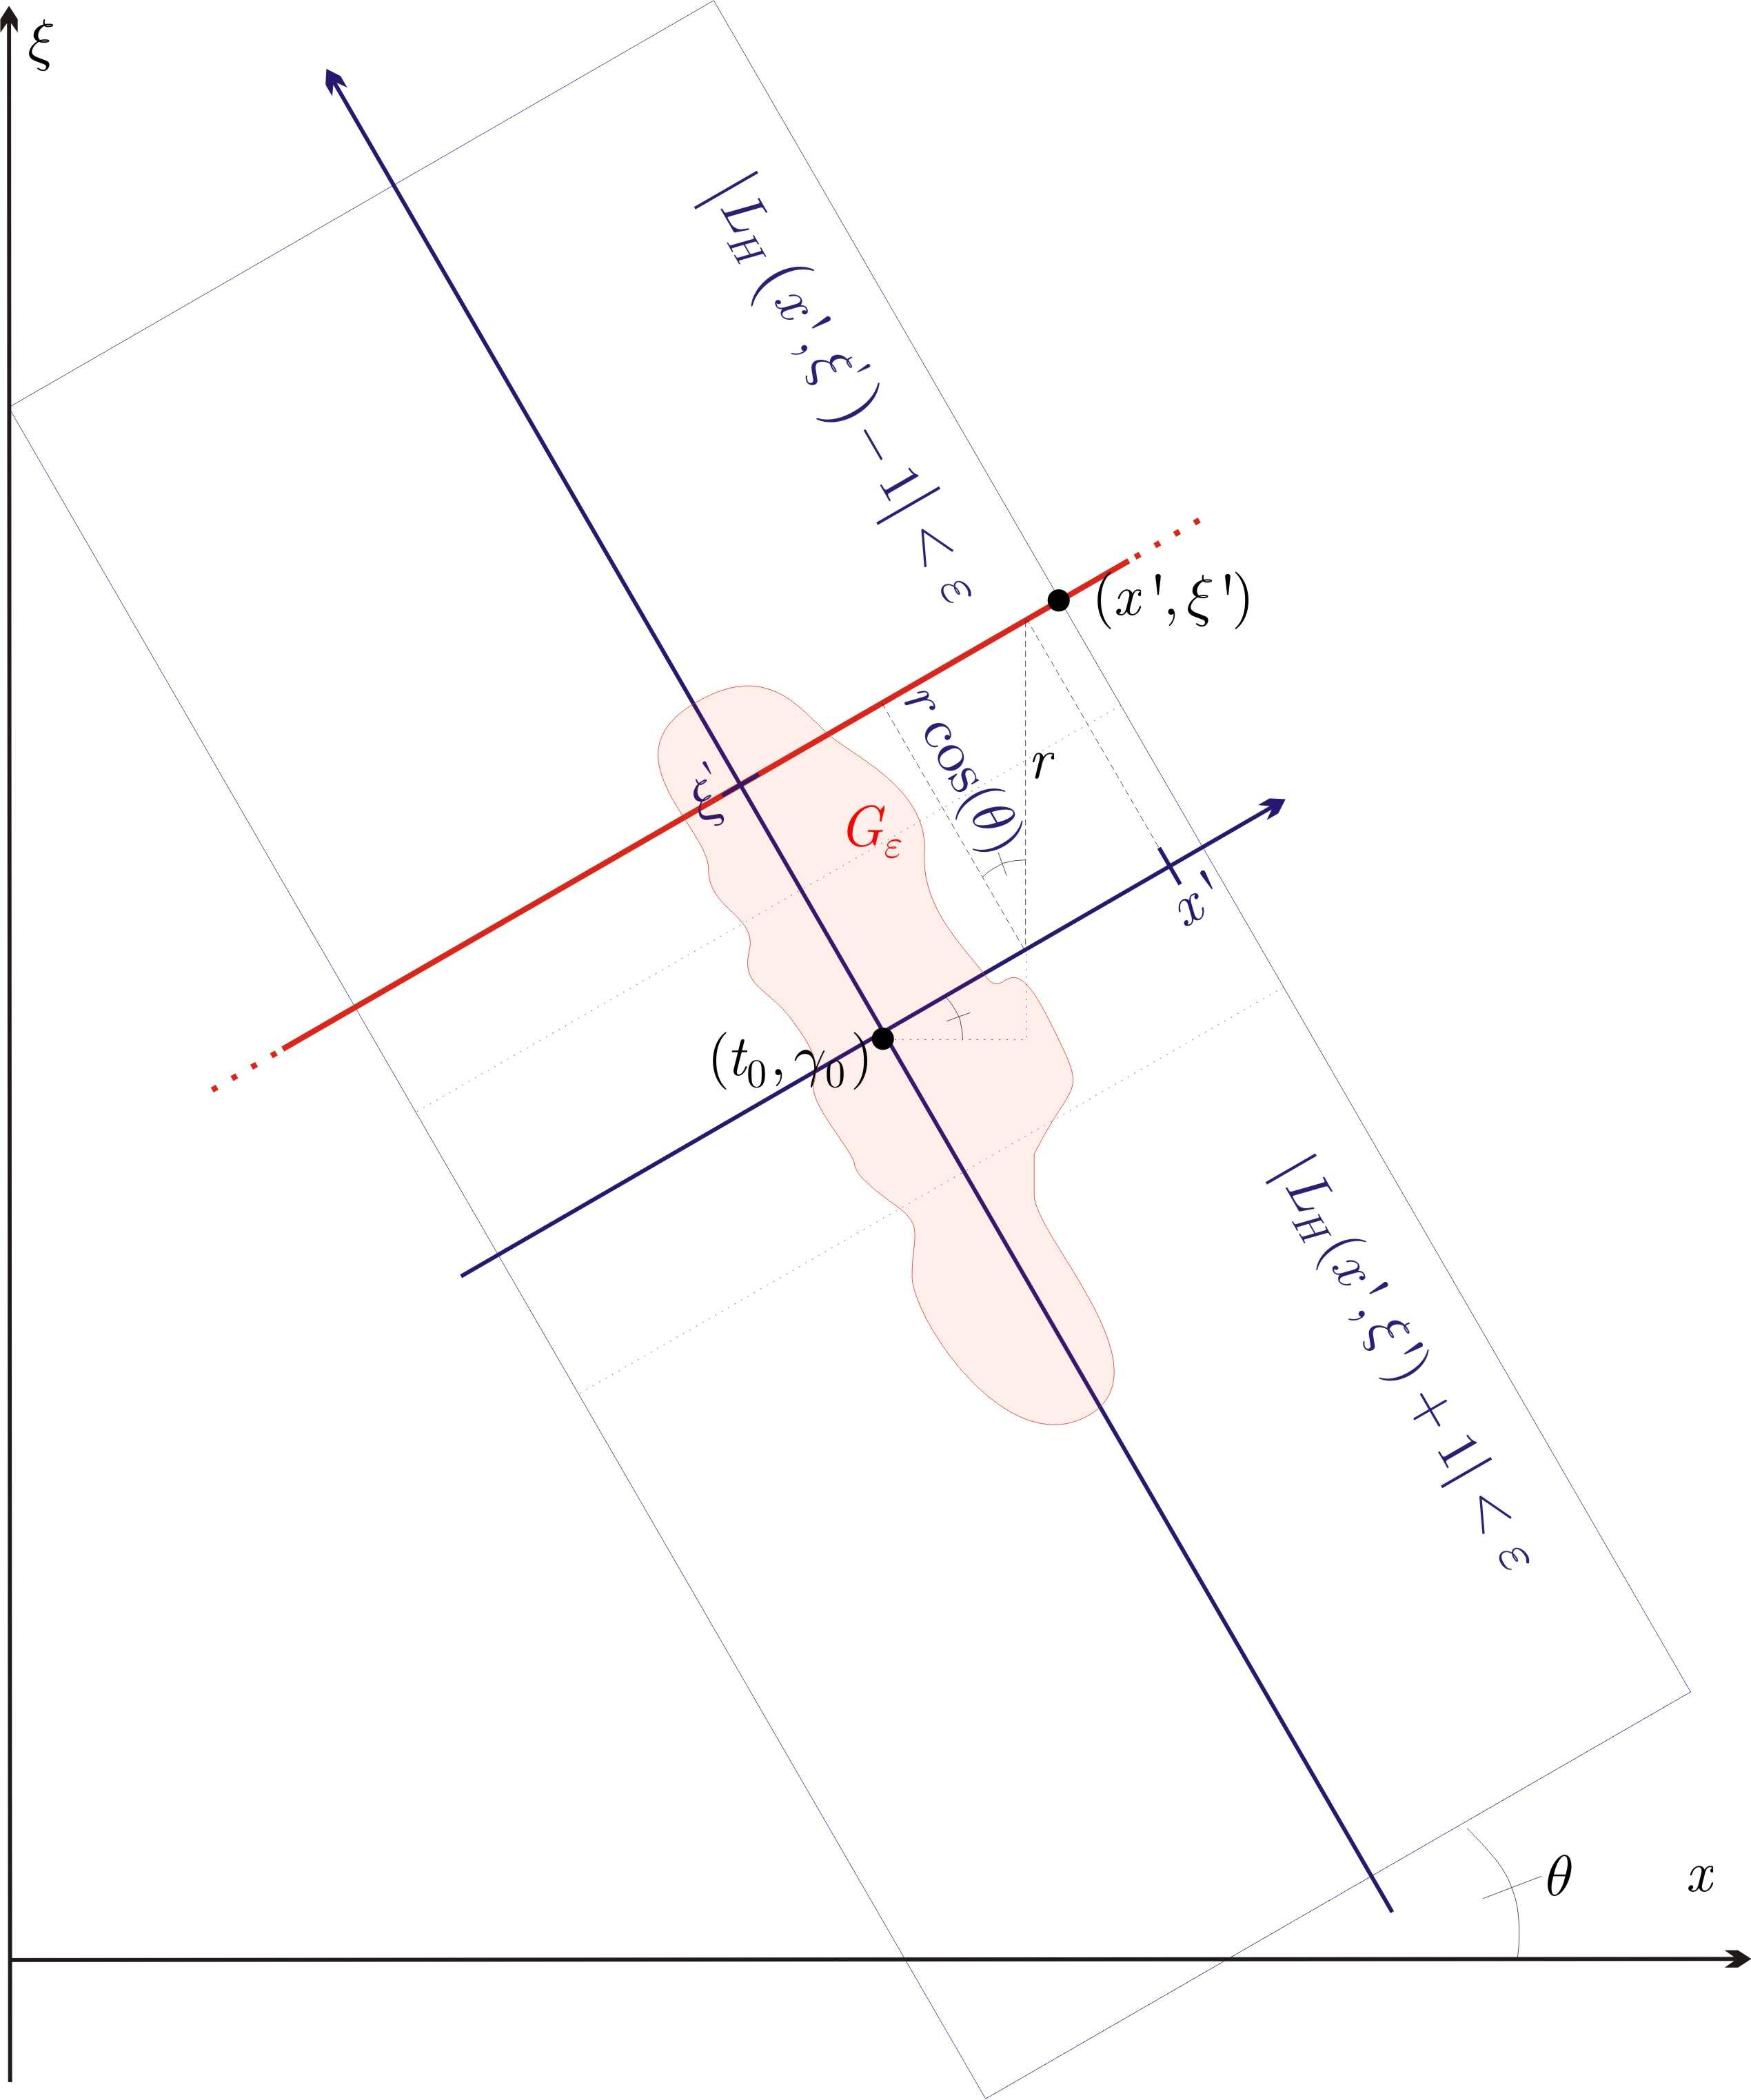
\includegraphics[width=7cm]{pfander.png}
     \caption{Construction of a channel spreading function whose operator causes a large distortion to a function
     with time--frequency $\epsilon$-support $G_\epsilon$.}
     \label{fig:pfander}
   \end{center}
 \end{figure}
% to reference it use ``Figure.~\ref{fig:xxx}''; the numbers will be computed automatically.

Within this realm, we derived estimates which relate the worst case
distortion of a function to the functions time--frequency
concentration and the channel operators spreading support (see
Figure~\ref{fig:pfander}). These results should, similarly to our
previous work on time invariant channels, allow us to show that OFDM
outperforms wavelet methods in mobile communication channels.

Further,  we continued our work on the modelling of narrowband
finite lifelength systems such as wireless radio communications by
smooth and compactly supported spreading functions. Our results were
used to derive a fast algorithm for computing the matrix
representation of a channel operator with respect to pulseshaped
OFDM bases \cite{GP06}.

\null {\emph{Operator/Channel Identification:}}  One of the key
problems in the design of elementary building blocks for mobile
communications is the incomplete knowledge of the ever--changing
transmission channels. The goal of operator/channel identification
is to obtain complete knowledge of a (channel-) operator by
observing the output caused by a single input signal.

Within the last years, we showed that classes of operators characterized by a bounded
spreading support region allow identification of its members if and only if the area of
the spreading support region is less than or equal to one, a phenomenon which is closely
related to Heisenberg's uncertainty principle~\cite{PW06,PW06b}. The theory, motivated by
communications engineering, has lead to the development of a sampling theory of operators
which is described in Section~\ref{mps:pfander}.

\null {\emph{Coding:}} Discrete, overcomplete Gabor systems can be
used to encode finite dimensional vectors in order to gain
robustness to errors introduced in  communications channels. In
\cite{KPR06}, we construct a large class of Gabor like equal norm
tight frames that are maximally robust to erasures. Further, we
discuss consequences of our findings to the theory of recovering and
storing signals which have sparse time--frequency representations.

%These results are further discussed in~\cite{KPR05}. The main
%focus of this paper are uncertainty principles for time--frequency
%representations of vectors in  finite dimensional vector spaces
%(Section~\ref{mps:pfander}).

%Possibly Channel matrix as picture
%
%% to include a figure, generate a file xxx.pdf and integrate the following lines
%\begin{figure}[ht]
%  \begin{center}
%   \includegraphics[width=10cm]{Pfander.pdf}
%    \caption{The caption of the figure}
%    \label{fig:xxx}
%  \end{center}
%\end{figure}
%% to reference it use ``Figure.~\ref{fig:xxx}''; the numbers will be computed automatically.
%
% Text ....
%
%
%\paragraph{Organization}
%% list the (research) events you have organized, if any,
%
%\begin{enumerate}
%\item  ....
%\item   ...
%\item  ...
%\end{enumerate}

\null G\"otz Pfander is also involved in  ``Applied Mathematics''
(Section~\ref{mps:pfander}).

\paragraph{Collaborations}
\begin{enumerate}
    \item {\sl International University Bremen}\\
          Prof. Harald Haas, Prof. Werner Henkel\\
          Design of OFDM systems for time--varying channels
    \item {\sl George Mason University, USA}\\
          Prof. David Walnut\\
          Operator sampling and channel measurements
    \item {\sl Numerical Harmonic Analysis Group and European Center
          for Time--Frequency Analysis, Vienna University, Austria}\\
          Prof. Hans Feichtinger, Prof. Karlheinz Gr\"ochenig\\
          Gabor analysis and applications to mobile communications
\end{enumerate}

\newpage
\paragraph{Grants}

\begin{enumerate}
    \item Funded by DFG, \emph {Analysis and design of COFDM multicarrier modulation techniques in view
          of transmission stability in time variant channels}, (September 2004 - December
          2006)
\end{enumerate}

%
%\paragraph{Patents}
%% list the grants you have received in 2005, if none have been received, plese delete this
%% subsection.
%\begin{enumerate}
%\item
%\item
%\end{enumerate}
%

%\paragraph{Awards, Prices}
%% list the grants you have received in 2005, if none have been received, plese delete this
%% subsection.
%\begin{enumerate}
%\item
%\item
%\end{enumerate}

%\paragraph{Publications}
% list the publications of 2005 (also accepted and in press), if none have been received, plese delete this
% subsection. Enter the publications into the SES publications database at
% http://kwarc.eecs.iu-bremen.de/ses-pubs/index.php and only reference them here.

%\begin{description}
 % \item[Journals]  Journal of Fourier Analysis and
 % Applications~
  %\nocite{LPW05,Pfa05}
 % \item[Submitted] IEEE Transactions on Information
%  Theory~
  %\nocite{PW051,GP05}
%\item[In preparation]
%\nocite{Pfa05b,KPR05}
%\end{description}


%\bibliographystyle{alpha}
%\bibliography{report-pfander-2005}

%\end{document}
%%% Local Variables:
%%% mode: latex
%%% TeX-master: "report"
%%% End:
